% !TeX document-id = {4a66a092-a797-425f-b588-c0b0f6bcb4d3}
% !TeX TXS-program:compile = txs:///lualatex | txs:///biber | txs:///lualatex | txs:///lualatex | txs:///view
\documentclass[landscape,paperwidth=48in,paperheight=36in,fontscale=0.3]{baposter}

\usepackage{times}
\usepackage{calc}
\usepackage{url}
\usepackage{graphicx}
\usepackage{diffcoeff}
\usepackage[intlimits]{mathtools}
\usepackage{nicematrix}
\usepackage{amsthm}
\usepackage{amssymb}
\usepackage{relsize}
\usepackage{multirow}
\usepackage{multicol}
\usepackage{booktabs}
\usepackage{microtype}

\usepackage[T1]{fontenc}
\usepackage{ae}
\usepackage{enumitem}
\usepackage{colortbl}
\usepackage{xcolor}
\usepackage{tcolorbox}
\usepackage[vlined]{algorithm2e}
\let\vec\mathbf
\setlength{\algomargin}{0pt}

\setlist[itemize]{leftmargin=*,nosep}
\setlength{\columnsep}{0.7em}
\setlength{\columnseprule}{0mm}

\setlist[enumerate]{leftmargin=2.3em,nosep}
\setlength{\columnsep}{0.5em}
\setlength{\columnseprule}{0mm}

\renewcommand{\familydefault}{\sfdefault}

% define colors
\newcommand{\highlight}[2][yellow]{\mathchoice%
  {\colorbox{#1}{$\displaystyle#2$}}%
  {\colorbox{#1}{$\textstyle#2$}}%
  {\colorbox{#1}{$\scriptstyle#2$}}%
  {\colorbox{#1}{$\scriptscriptstyle#2$}}}%
  
\definecolor{ctitle}{HTML}{000000}
\definecolor{mypurple}{RGB}{223, 204, 251}
\definecolor{imptext}{RGB}{103, 65, 136} 
\definecolor{rowcolor}{RGB}{209, 233, 246}
\definecolor{subtitlecolor}{RGB}{11, 47, 159}
\definecolor{mathcolor}{RGB}{209, 233, 246}
\definecolor{mathcolor2}{RGB}{238, 202, 213}

\difdef {f,fp,s,sp} {|}{
    outer-Ldelim =\left.,
    outer-Rdelim=\right|,
    sub-nudge=0mu
}

\theoremstyle{definition}
\newtheorem{definition}{Definition}
\newtheorem{example}{Example}
\newtheorem{theorem}{Theorem}

\begin{document}

\begin{poster}{
    grid=false,
    columns=100,
    colspacing=0.7em,
    headerColorOne=mypurple,
    borderColor=mypurple,
    textborder=faded,
    headerborder=open,
    headershape=roundedright,
    headershade=plain,
    background=none,
    bgColorOne=cyan!10!white,
    headerheight=0.15\textheight}
    {
    \makebox[0.01\textwidth]{}
    
\includegraphics[width=0.08\linewidth]{logo/logounmsmcolor}\hspace{.5cm}
    
\includegraphics[width=0.08\linewidth]{logo/escudouni}
    }
    % Title
    {
    \\[0.2em]\sc\huge\bf Numerical solution for differential equations of Lane-Emden type \\[0.1em]
    by Adomian decomposition and integration methods
    }
    % Authors
    {
    \vspace{0.2em} Matihus Alberth Molina Larios$^{\clubsuit1}$ \enspace Carlos Alonso Aznarán Laos$^{\clubsuit2}$ \\[0.1em]
    {$^1$Facultad de Ciencias Matemáticas, Universidad Nacional Mayor de San Marcos \\[0.1em] \enspace$^2$Facultad de Ciencias, Universidad Nacional de Ingeniería \\[0.1em]
    \(\clubsuit\) indicates equal contribution}
    }
    % University logo
    {
    \makebox[0.01\textwidth]{}
    
\includegraphics[width=0.22\linewidth]{logo/FlyerE}
    }

    \headerbox{\bf\color{ctitle}Adomian Decomposition Method}{name=summary,column=0,row=0,span=30}{
    \small
    \setlength{\abovedisplayskip}{3pt}
    \setlength{\belowdisplayskip}{3pt}
    \setlength{\parskip}{2pt}

    The general operator equation is written as
    \begin{equation}\label{eq:generaloperator}
        Lu+Ru+Nu=g.
    \end{equation}
    Where the operators represent
    \vspace*{-\baselineskip}\setlength\belowdisplayshortskip{0pt}
    \begin{multicols}{2}
        \begin{itemize}
            \setlength\itemsep{0em}
            \item $L$: Highest order derivative term.

            \item $R$: Lower order derivative terms.

            \item $N$: Nonlinear terms.

            \item $g$: Source term.
        \end{itemize}
    \end{multicols}
    \vspace*{-\baselineskip}\setlength\belowdisplayshortskip{0pt}
    Applying $L^{-1}$ to~\eqref{eq:generaloperator}, we obtain
    \begin{equation*}
        u=
        \phi+
        L^{-1}g-
        L^{-1}Ru-
        L^{-1}Nu.
    \end{equation*}
    \begin{definition}[\bfseries Adomian polynomials $A_{n}$ and $L^{-1}$ for Lane-Emden type]
        \begin{align*}
            \forall n\in\mathbb{N}\cup\left\{0\right\}:
            A_{n}                    & \coloneqq
            \frac{1}{n!}
            \diff*[n]{
                \left[
                    N\left(
                    \sum_{i=0}^{\infty}
                    \lambda^{i}
                    u_{i}
                    \right)
            \right]_{\lambda=0}}{\lambda}.       \\
            L^{-1}\left(\cdot\right) & \coloneqq
            \int_{0}^{\xi}
            s^{-2}
            \left(
            \int_{0}^{s}
            t^{2}\left(\cdot\right)
            \dl t
            \right)
            \dl s.
        \end{align*}
    \end{definition}
    Decomposing $u=\sum\limits_{n=0}^{\infty}u_{n}$,
    the recursive scheme is
    \begin{equation}\label{eq:adm_system}
        \left\{
        \begin{aligned}
            \forall n\in\mathbb{N}\cup\left\{0\right\}:
            u_{n+1} & =
            -L^{-1}Ru_{n}-L^{-1}A_{n}. \\
            u_{0}   & =
            \phi+L^{-1}g.
        \end{aligned}
        \right.
    \end{equation}
    }

    \headerbox{\bf\color{ctitle}ODE Integration for a Singular IVP}{name=method,column=30,row=0,span=25}{
        % Consider the problem of find the numerical solution of the system non-stiff singular initial value problem
        % \begin{equation*}
        %     \diff{u}{\xi}=
        %     f\left(\xi, u\right),\quad
        %     u\left(\xi_{0}\right)=u_{0}\in\mathbb{R}^{d},\quad
        %     \xi\in\left(t_{\text{initial}},t_{\text{final}}\right).
        % \end{equation*}
        % It is an explicit seventh-order Runge-Kutta method
        % (integrated only at orders 4 and 5), with local error estimation and step size control
        \begin{center}
            \scshape\bfseries
            Butcher table for Dormand-Prince RK5(4)7M
        \end{center}
        \vspace*{-.5\baselineskip}\setlength\belowdisplayshortskip{0pt}
        \begin{equation*}\NiceMatrixOptions{cell-space-limits=1pt}
            \begin{NiceArray}[t]{c|cccccc}
                \toprule
                c_{i}         & a_{ij}                                                                                                                            \\
                \midrule
                0                                                                                                                                                 \\
                \dfrac{1}{5}  & \dfrac{1}{5}                                                                                                                      \\
                \dfrac{3}{10} & \dfrac{3}{40}          & \dfrac{9}{40}                                                                                            \\
                \dfrac{4}{5}  & \dfrac{44}{45}         & -\dfrac{56}{15}        & \dfrac{32}{9}                                                                   \\
                \dfrac{8}{9}  & \dfrac{19372}{6561}    & -\dfrac{25360}{2187}   & \dfrac{64448}{6561} & -\dfrac{212}{729}                                         \\
                1             & \dfrac{9017}{3168}     & -\dfrac{355}{33}       & \dfrac{46732}{5247} & \dfrac{49}{176}   & -\dfrac{5103}{18656}                  \\
                1             & \dfrac{35}{384}        & 0                      & \dfrac{500}{1113}   & \dfrac{125}{192}  & -\dfrac{2187}{6784}  & \dfrac{11}{84} \\
                \bottomrule
                              & b^{\left(5\right)}_{i} & b^{\left(4\right)}_{i} &                     &                   &                      &
            \end{NiceArray}
        \end{equation*}
        \vspace*{-\baselineskip}\setlength\belowdisplayshortskip{0pt}
        \begin{align*}
            b^{\left(5\right)} & =
            \begin{bNiceMatrix}[columns-width=1mm]
                \dfrac{35}{384} & 0 & \dfrac{500}{1113} & \dfrac{125}{192} & -\dfrac{2187}{6784} & \dfrac{11}{84} & 0
            \end{bNiceMatrix} . \\
            b^{\left(4\right)} & =
            \begin{bNiceMatrix}[columns-width=1mm]
                \dfrac{5179}{57600} & 0 & \dfrac{7571}{16695} & \dfrac{393}{640} & -\dfrac{92097}{339200} & \dfrac{187}{2100} & \dfrac{1}{40}
            \end{bNiceMatrix}.
        \end{align*}
        % \textbf{Illustration}
        % \begin{minipage}{0.99\linewidth}
        %     \centering
        %     \includegraphics[width=0.45\linewidth]{example-image}
        % \end{minipage}
    }

    \headerbox{\bf\color{ctitle}Introduction}{name=results,column=55,row=0,span=45}{

        \textbf{Given:}
        \begin{equation*}
            \left.\begin{aligned}
                \diff{P}{r} & = -\frac{GM\rho}{r^{2}}.                \\
                \diff{M}{r} & = 4\pi r^{2}\rho.                       \\
                P           & = K{\left(\rho\right)}^{1+\frac{1}{n}}.
            \end{aligned}\right\}
            \implies
            \begin{aligned}
                \frac{1}{r^{2}}
                \diff*{
                    \left(
                    \frac{r^{2}}{\rho}\diff{P}{r}
                    \right)
                }{r}=
                -4\pi G \rho. \\
                \text{See the model derivation.}
            \end{aligned}
        \end{equation*}
        \textbf{Goal:}
        \begin{equation*}
            \text{Numerical solutions Lane-Emden ODE when }n\neq 0,1,5.
        \end{equation*}

        \textbf{Existing methods:}
        \begin{enumerate}
            \item Transform 2nd ODE to 1st ODE system.

            \item Adomian decomposition method.

            \item Differential transform method.
        \end{enumerate}
        \textbf{Contributions:}
    }

    % % BOX 4: EXISTENCE AND UNIQUENESS
    \headerbox{\bf\color{ctitle}Existence, Uniqueness and Error Estimation}{name=algorithm,column=0,row=0.43,span=30}{
        \small
        \setlength{\abovedisplayskip}{3pt}
        \setlength{\belowdisplayskip}{3pt}
        \setlength{\abovedisplayshortskip}{1pt}
        \setlength{\belowdisplayshortskip}{1pt}

        \begin{theorem}[\colorbox{mathcolor}{\bfseries Existence and Uniqueness}]
            Let $m\in\mathbb{N}$.
            If $g\in C^{1}$,
            then $\forall\alpha\in\mathbb{R}$,
            $\exists! u\in C^{2}\left(\mathbb{R},\mathbb{R}\right)$ such that
            \begin{equation}
                \left\{
                \begin{aligned}
                    \diff*{\left(\xi^{m-1}\diff{u}{\xi}\right)}{\xi} & =
                    \xi^{m-1} g\left(u,\xi\right).                       \\
                    u\left(0\right)=\alpha,\quad \diff.|.{u}{\xi}[0] & =
                    0.
                \end{aligned}
                \right.\label{eq:1}
            \end{equation}
        \end{theorem}

        \begin{proof}
            Let $v\coloneqq\diff{u}{\xi}$. The problem~\eqref{eq:1}
            implies the integral equation
            \vspace*{-.5\baselineskip}\setlength\belowdisplayshortskip{0pt}
            \begin{equation*}
                \left\{
                \begin{aligned}
                    \diff{u}{\xi}                        & =
                    v.                                       \\
                    \diff*{\left(\xi^{m-1}v\right)}{\xi} & =
                    \xi^{m-1}
                    g\left(u,\xi\right).                     \\
                    u\left(0\right)=\alpha,
                    v\left(0\right)                      & =
                    0.
                \end{aligned}
                \right.\iff
                \left\{
                \begin{aligned}
                    u\left(\xi\right) & =
                    \alpha+
                    \int_{0}^{\xi}
                    v\left(t\right)\dl t. \\
                    v\left(\xi\right) & =
                    \frac{1}{\xi^{m-1}}
                    \int_{0}^{\xi}
                    t^{m-1}
                    g\left(u,t\right)\dl t.
                \end{aligned}
                \right.
            \end{equation*}
            Let $\varepsilon>0$, $X_{\varepsilon}= C([0,\varepsilon])\times C([0,\varepsilon])$.\newline
            For $(u,v)\in X_{\varepsilon}$:
            ${\|(u,v)\|}_{\varepsilon}= \max \left\{ \max_{0\leq t\leq\varepsilon}|u(t)|, \max_{0\leq t\leq\varepsilon}|v(t)| \right\}$.\newline
            \textbf{Claim:} $\left(X_{\varepsilon},{\left\|\cdot\right\|}_{\varepsilon}\right)$ is a Banach space.\newline
            Define $T\colon K \longrightarrow K$ over closed set $K\subset X$:
            \begin{align*}
                \left(u,v\right)
                \longmapsto
                \left(
                \alpha+
                \int_{0}^{\xi}
                v\left(t\right)\dl t,
                \frac{1}{\xi^{m-1}}
                \int_{0}^{\xi}
                t^{m-1}g\left(u,t\right)\dl t
                \right).
            \end{align*}
        \end{proof}

        \begin{theorem}[\colorbox{mathcolor2}{\bfseries Error bound}]
            Let $u\in C^{n+1}\left(\left[0,1\right]\right)$ the exact
            solution of~\eqref{eq:1} and $u_{n}=\sum_{i=0}^{n}c_{i}t^{i}$
            their $n$-th order approximation.
            Then,
            \begin{equation*}
                \left\|u\left(t\right)-u_{n}\left(t\right)\right\|_{\infty}\leq
                \frac{M}{\left(n+1\right)!}+
                \max_{0\leq i\leq n}
                \left|a_{i}\right|,
            \end{equation*}
            where
            \begin{math}\displaystyle
                M=
                \max_{0\leq t\leq 1}
                \left|
                u^{\left(n+1\right)}\left(t\right)
                \right|
            \end{math}
            and
            \begin{math}\displaystyle
                a_{i}=
                \sum_{i=0}^{n}
                \left[
                    \frac{u^{\left(i\right)}\left(0\right)}{i!}-
                    c_{i}
                    \right]
            \end{math}.
        \end{theorem}
    }

    % % BOX 5: IS CHM NECESSARY?
    % \headerbox{\bf\color{ctitle}Is \textsc{CHM} Necessary?}{name=method,column=1,row=0.4,span=2,boxpadding=0.45em}{
    %     \includesvg[width=0.4\linewidth]{qrcode.svg}
    % }

    % % BOX 6: RESULTS
    \headerbox{\bf\color{ctitle}Numerical solutions for Lane-Emden type}{name=method,column=55,row=0.45,span=45,boxpadding=0.45em}{
        \begin{minipage}[t]{0.5\linewidth}
            \centering
            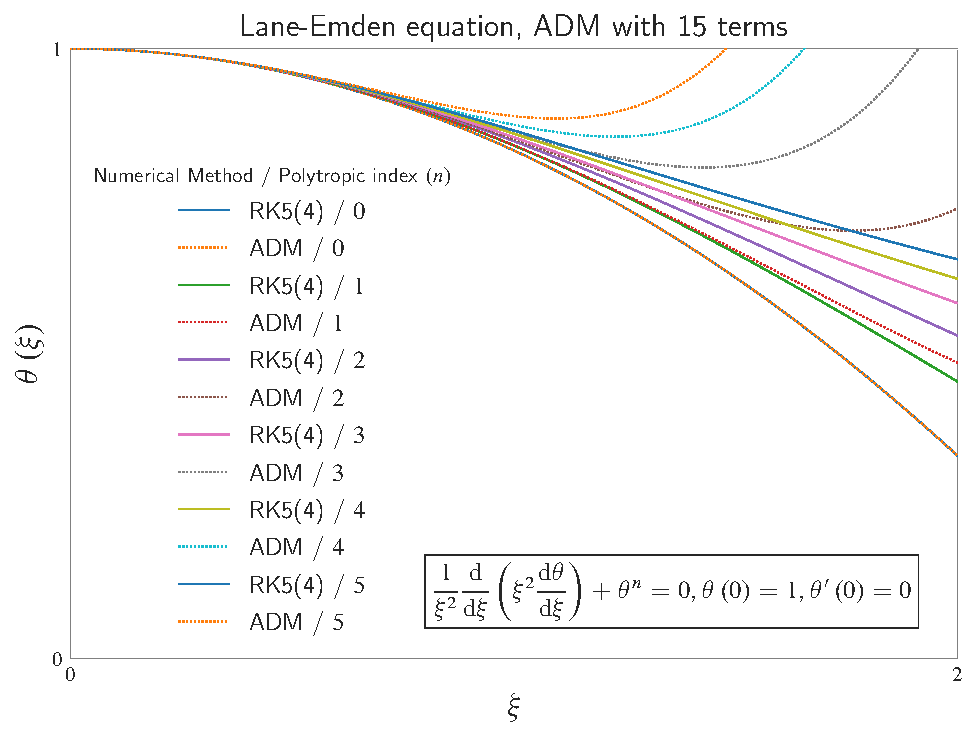
\includegraphics[width=\linewidth]{lane_emden}
            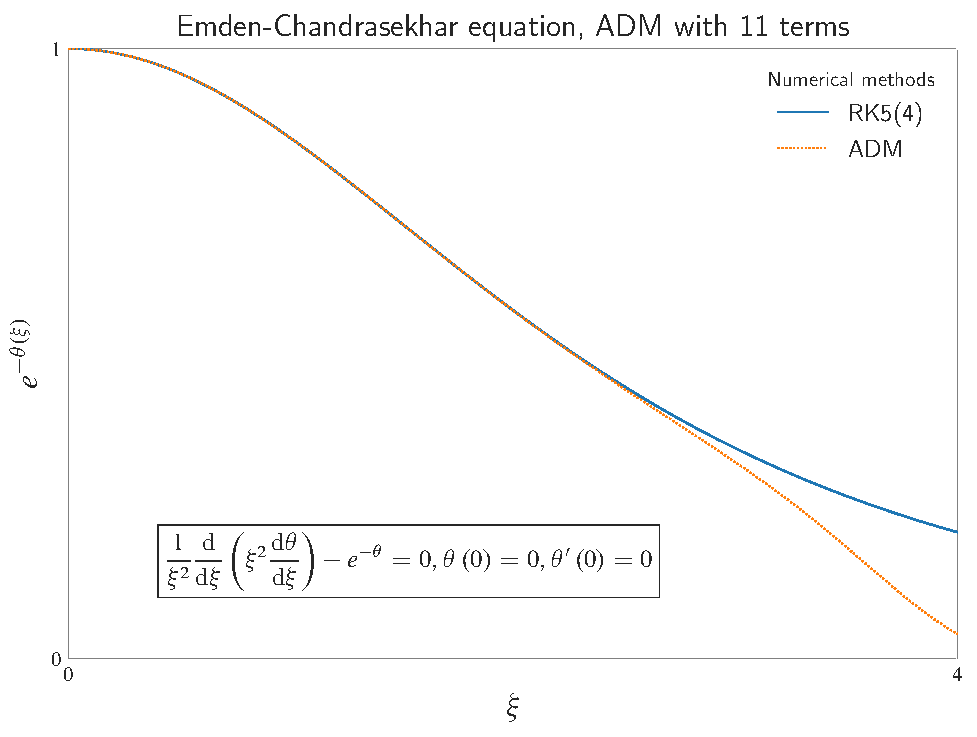
\includegraphics[width=\linewidth]{emden_chandrasekhar}
        \end{minipage}
        \begin{minipage}[t]{0.5\linewidth}
            \centering\vspace{-5.87cm}
            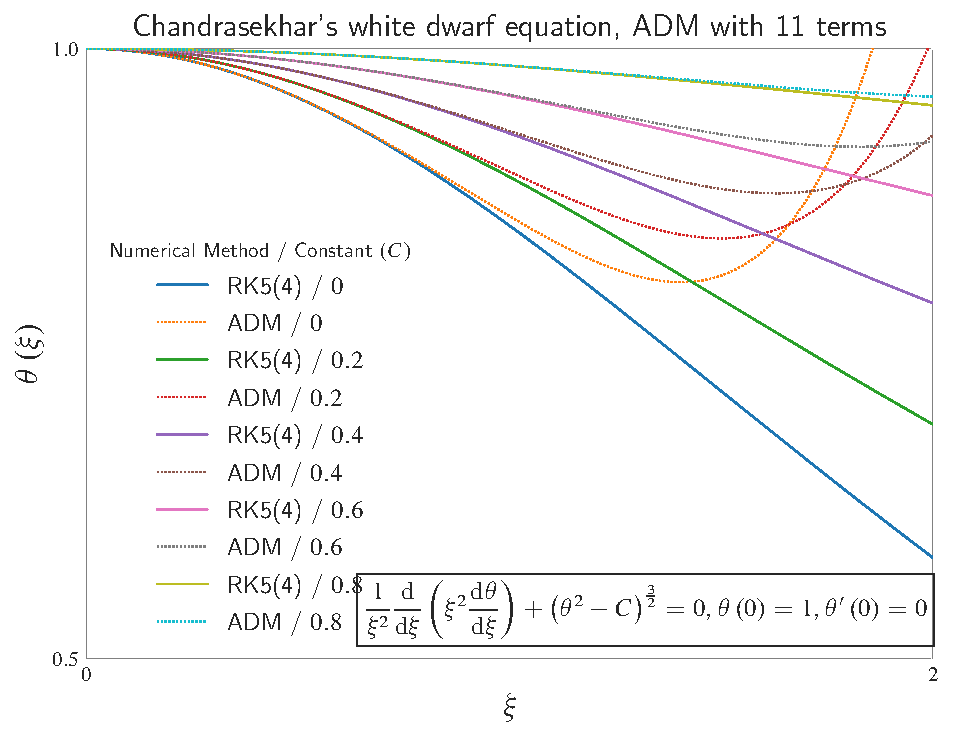
\includegraphics[width=\linewidth]{white_dwarf}
            
\includegraphics[width=.65\linewidth]{qrcode.pdf}

            Explore
        \end{minipage}
    }

\end{poster}
\end{document}